\documentclass{standalone}
\usepackage{xr-hyper}
\usepackage{hyperref}
\externaldocument[C3-]{Chapter3}
\begin{document}
\chapter{Data Analysis}
\label{Data Analysis}
As discussed in Chapter\ref{C3-Inertial Measurement Unit} in the Error section(\ref{C3-Error} on page \pageref{C3-Error}). IMU, during measurement suffer from accumulated error.\pageref{C3-Error}\\
The measurement along the pathway of road surface consists of a sampling of measurements at specific time intervals (usually in the order of milliseconds).So the road profile can be seen as an electronically acquired digital signal and consequently it is necessary clean up the signal from the noise\footnote{An unknown modifications that a signal may suffer during capture}, it may also be useful to delete certain information in the signal that is not of interest, or correct it from the drift (\ref{C3-Error}).\\


\noindent This cleaning procedure, also called filtering,it is used in the theory of signal analysis.
It is an essential aspect in the evaluation of the profile, \cite{little_book}. In brief, a digital filter represents a procedure that transforms a series of numbers into a new series of numbers, \cite{little_book}.\\
From the measurement obtained by the sensors, particular attention is given to the vertical acceleration signal and to the rotation vectors. \\
The rotation vectors will be useful for reorienting the signals obtained from the smartphone\cite{Andro} respect to the vehicle axes, while the vertical acceleration signal will be subject to various filtering operations depending on the final index to be obtained.\\\\
First of all, it is necessary to pay some attention to some dynamics\footnote{branch of mechanics that deals with the study of the motion of bodies and their causes or, more concretely, of the circumstances that determine and modify it} physical principles , about the operations that can be done, on the acceleration signal to get the position and vice-versa.\\\\
Given a position versus time of an object, $x(t)$, the velocity, $v(t)$, can be found by taking the first derivative.\\
\begin{center}
{\large $v(t) = \dfrac{dx}{dt}$}
\end{center}
Acceleration, $a(t)$, can be found by taking the second derivative of position or first
derivative of velocity.
\begin{center}
{\large $a(t) = \dfrac{d^{2}x}{dt^{2}} = \dfrac{dv}{dt}$}
\end{center}
However, is interesting to reverse this process and find the position signal given an acceleration signal. To do that, a double integration must be performed on the acceleration signal.
In principle, using double integration on an acceleration signal to get a position signal, the initial position and initial velocity must be known. After the first integration, the initial velocity should be added to the result, as the initial position should be added after the second integration. These operations are illustrated in the following equations
\begin{center}
\begin{equation}
 {\large v(t) = v(t_{0}) + \int_{t_{0}}^{t} \! a(\tau) \, \mathrm{d}\tau}
\end{equation}

Where: \\
\begin{table}[ht]
\centering
    \begin{tabular}{ | l | l |}
    
    \hline
    Symbol & Description \\ \hline
   \quad  $t_{0}$ & Initial Time \\ \hline
	   \quad  $v(t_{0})$ & Initial Velocity\\  
\hline 
    \end{tabular}
\end{table}
\end{center}

\noindent To get the position signal from velocity, is used the followed formula:
\begin{center}
\begin{equation}
 {\large x(t) = x(t_{0}) + \int_{t_{0}}^{t} \! v(\tau) \, \mathrm{d}\tau.}
\end{equation}

Where: \\
\begin{table}[ht]
\centering
    \begin{tabular}{ | l | l |}
    
    \hline
    Symbol & Description \\ \hline
   \quad  $t_{0}$ & Initial Time \\ \hline
	   \quad  $x(t_{0})$ & Initial Position \\  
\hline 
    \end{tabular}
\end{table}
\end{center}
\noindent Therefore, for a double integration of the acceleration, the two initial
conditions (velocity and position) must be known to avoid integration errors. However,
the only way to get these initial conditions is through direct measurement, which is often
impractical or unobtainable. By  data filtering, it is developed an approach that does not require knowledge of initial conditions.\\
To perform a numerical integration it is necessary to choose one integration algorithm of the many existing. 
The acceleration signal is sampled, making it a discrete function of time having a sampling frequency, $f_{s}$, associated with it. The easiest way to perform numerical integration is to use the rectangular integration method. This method uses an accumulator to sum all past sampled inputs and the current input sample and divide by the sampling rate. Rectangular integration is represented by the following difference equation:

\begin{center}
$y(n) = \dfrac{1}{f_{s}} \sum_{k=0}^{n} x(n-k) = y(n-1) + \dfrac{1}{f_{s}} x(n)$
\end{center}

\noindent Another numerical integration method uses the trapezoidal rule. 
The results are more precise with this method than the rectangular method. The difference equation for trapezoidal integration is:

\begin{center}
$y(n) = y(n-1) + \dfrac{1}{2 f_{s}}[x(n-1) + x(n)], n > 0$
\end{center}

The figure below show the difference using both methods.

\vspace{0.35cm}
\begin{figure}[ht]
\centering
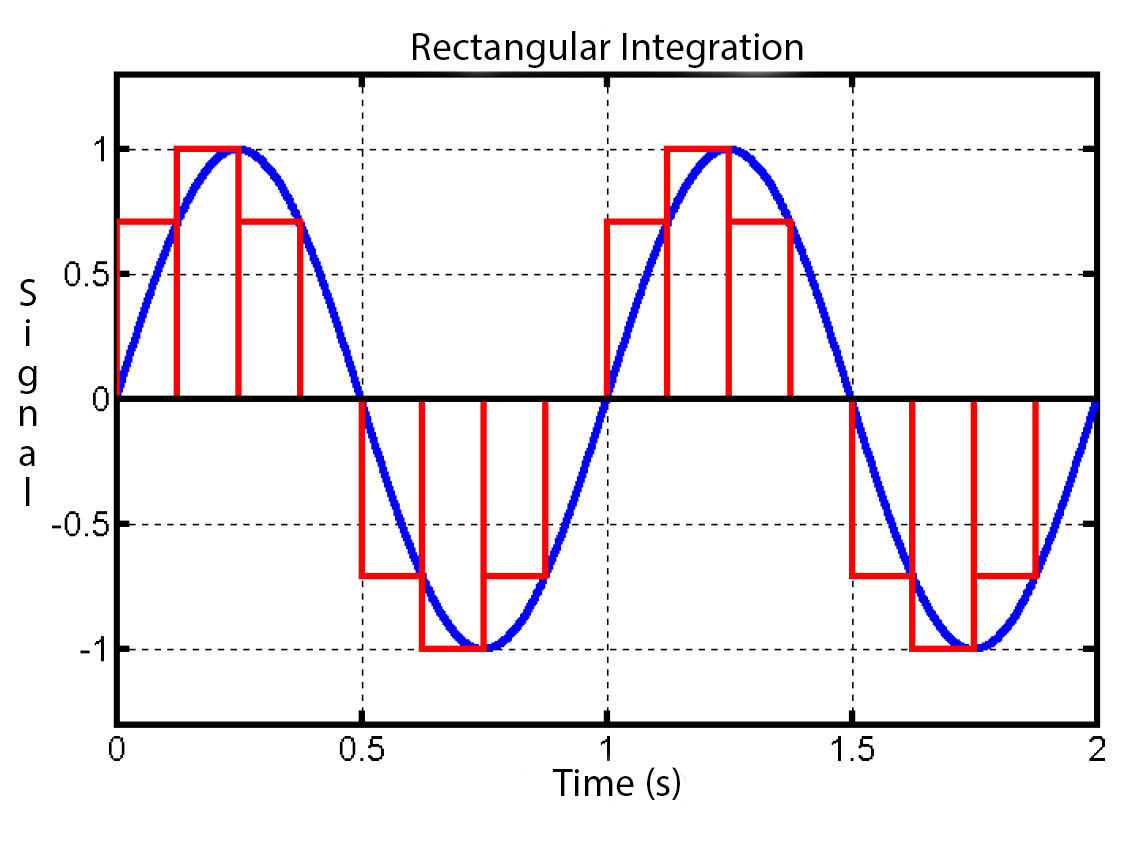
\includegraphics[scale=0.55]{RectangularInte}
\hspace{0.5cm}
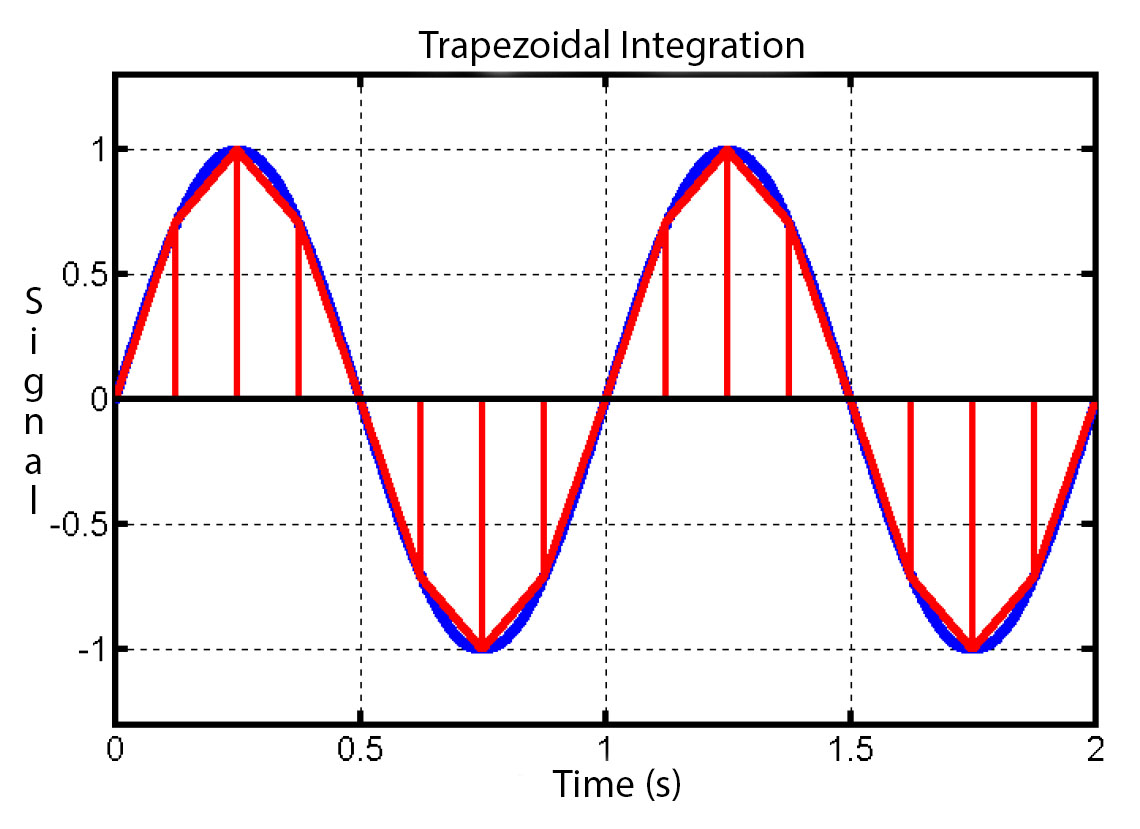
\includegraphics[scale=0.55]{TrapezoidalIntegration}
\caption{Integration using Rectangular (left) and Trapezoidal (right) methods of Sine Wave.}
\label{fig:Rectangular and Trapezoidal Integration}
\end{figure}

\noindent The integration was carried out using the trapezoidal method by the MATLAB suite. But without adequate cleaning of the signal, the result presents very error, caused by the drift and noise. \\
Various signal cleanup procedures will be discussed. The figure below shows the result of a raw signal integration using trapezoidal method.

\begin{figure}
  \centering
  \subfloat[Acceleration]{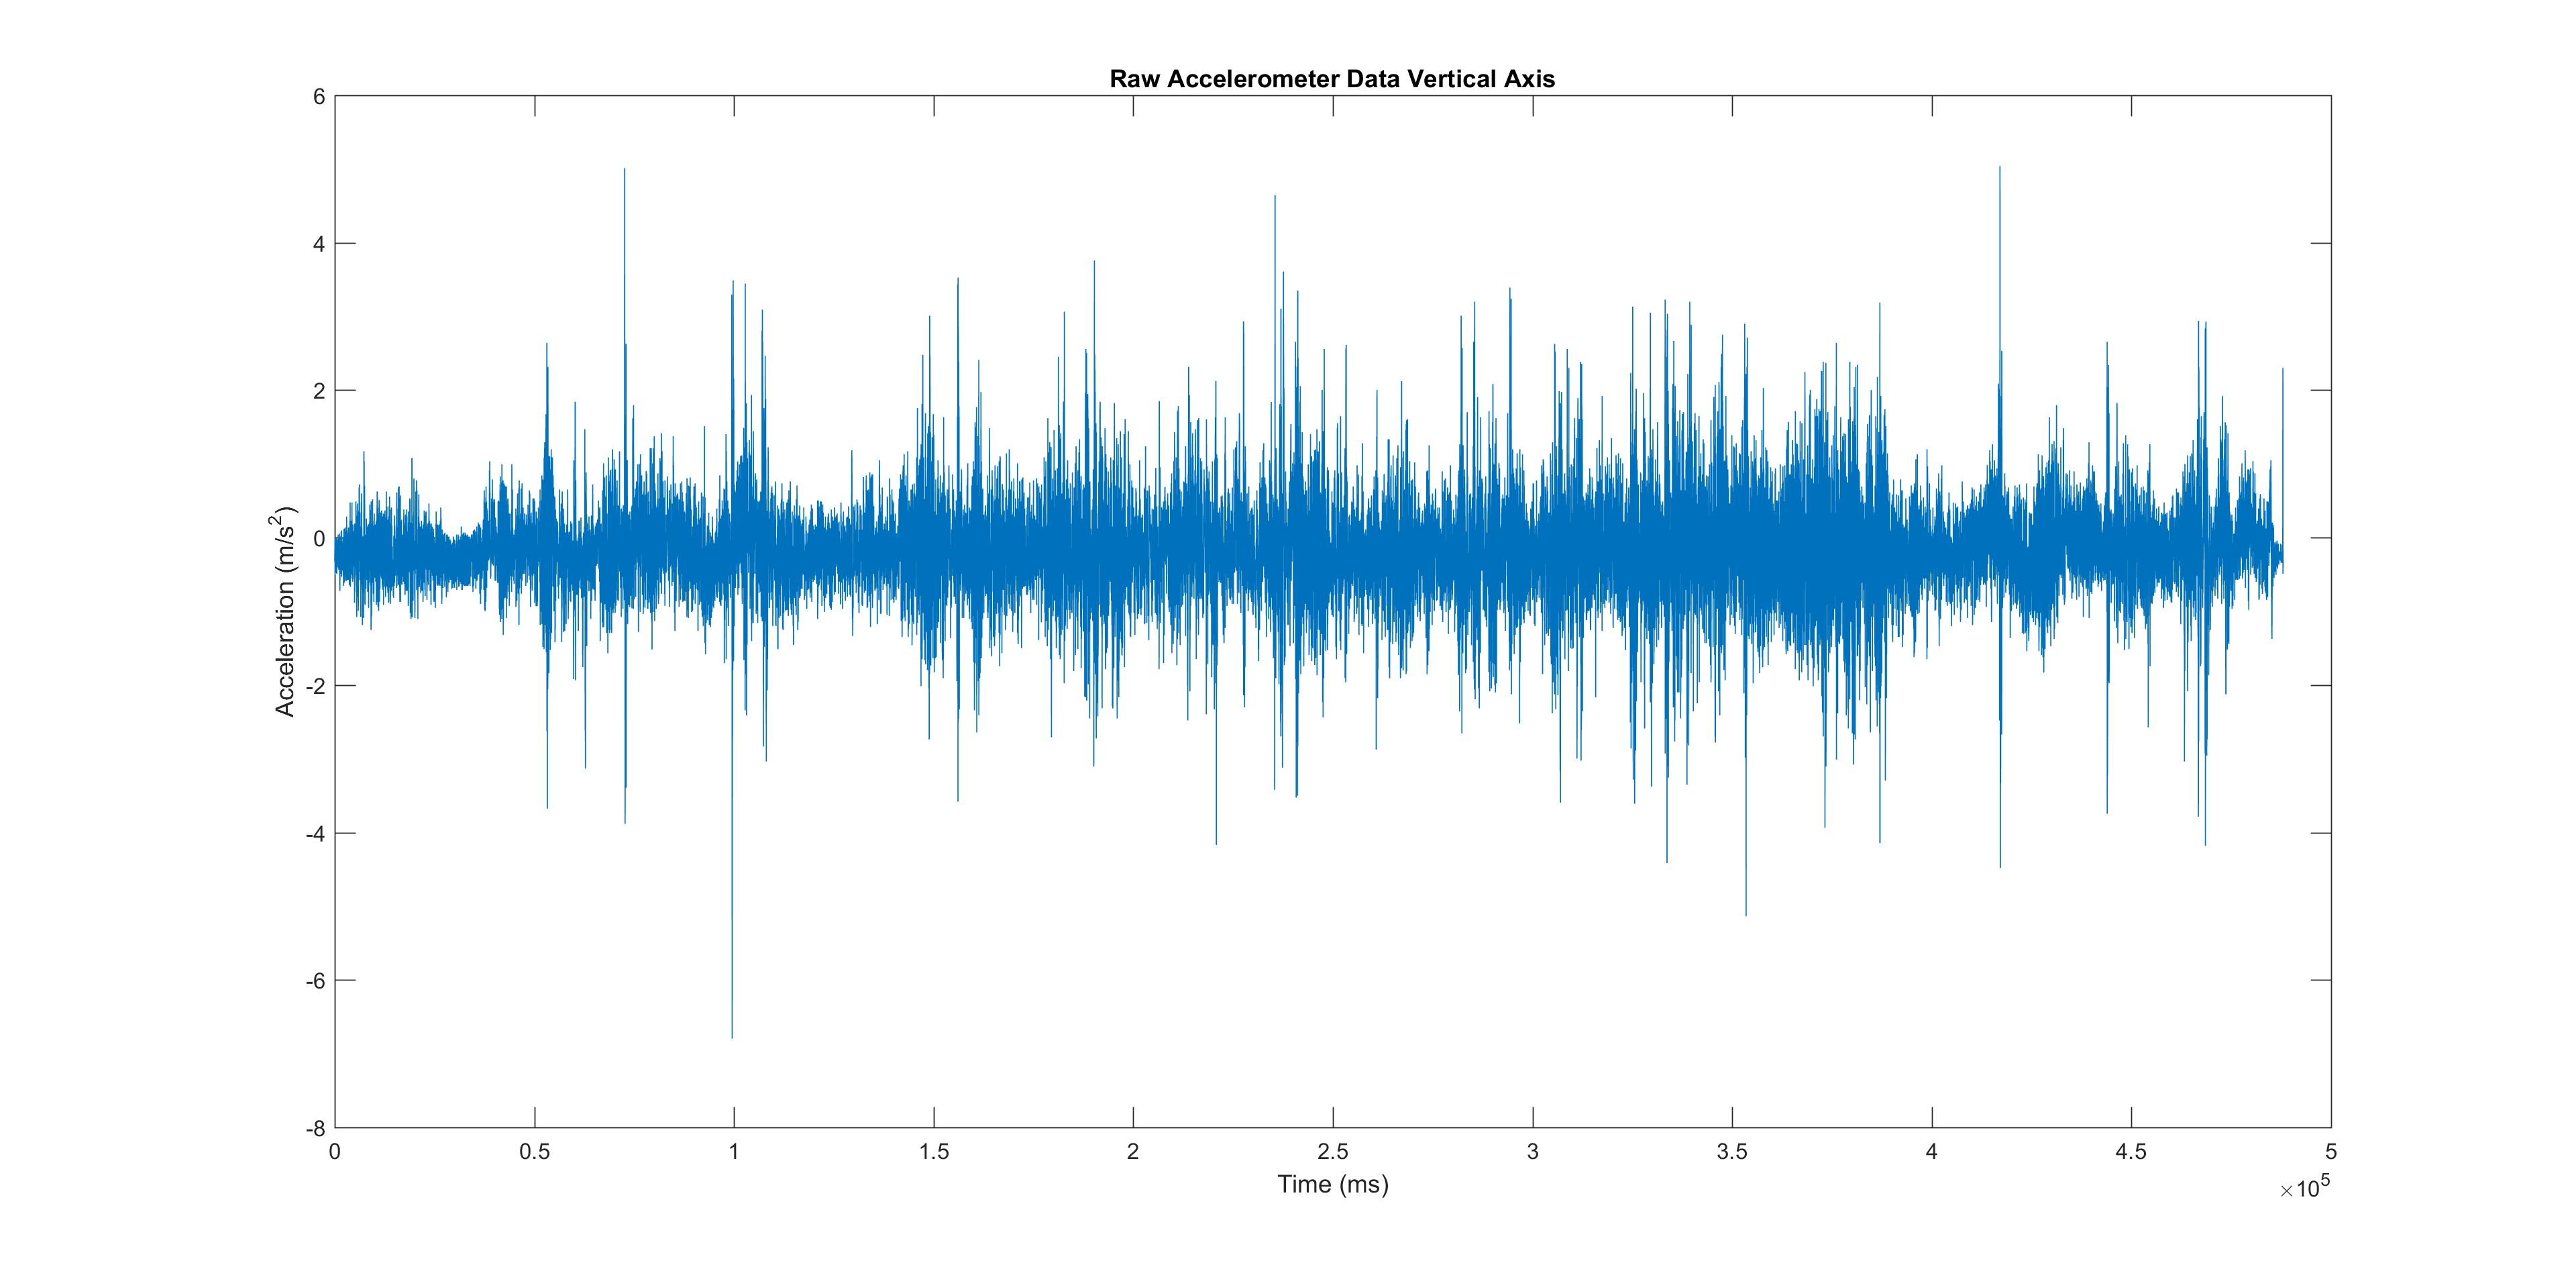
\includegraphics[scale=0.11]{RawAccelerometer}\label{fig:Raw Accelerometer}}  
  
  \subfloat[Velocity]{\includegraphics[scale=0.11]{VelocityIntegration}\label{fig:Velocity}}

  \subfloat[Displacement]{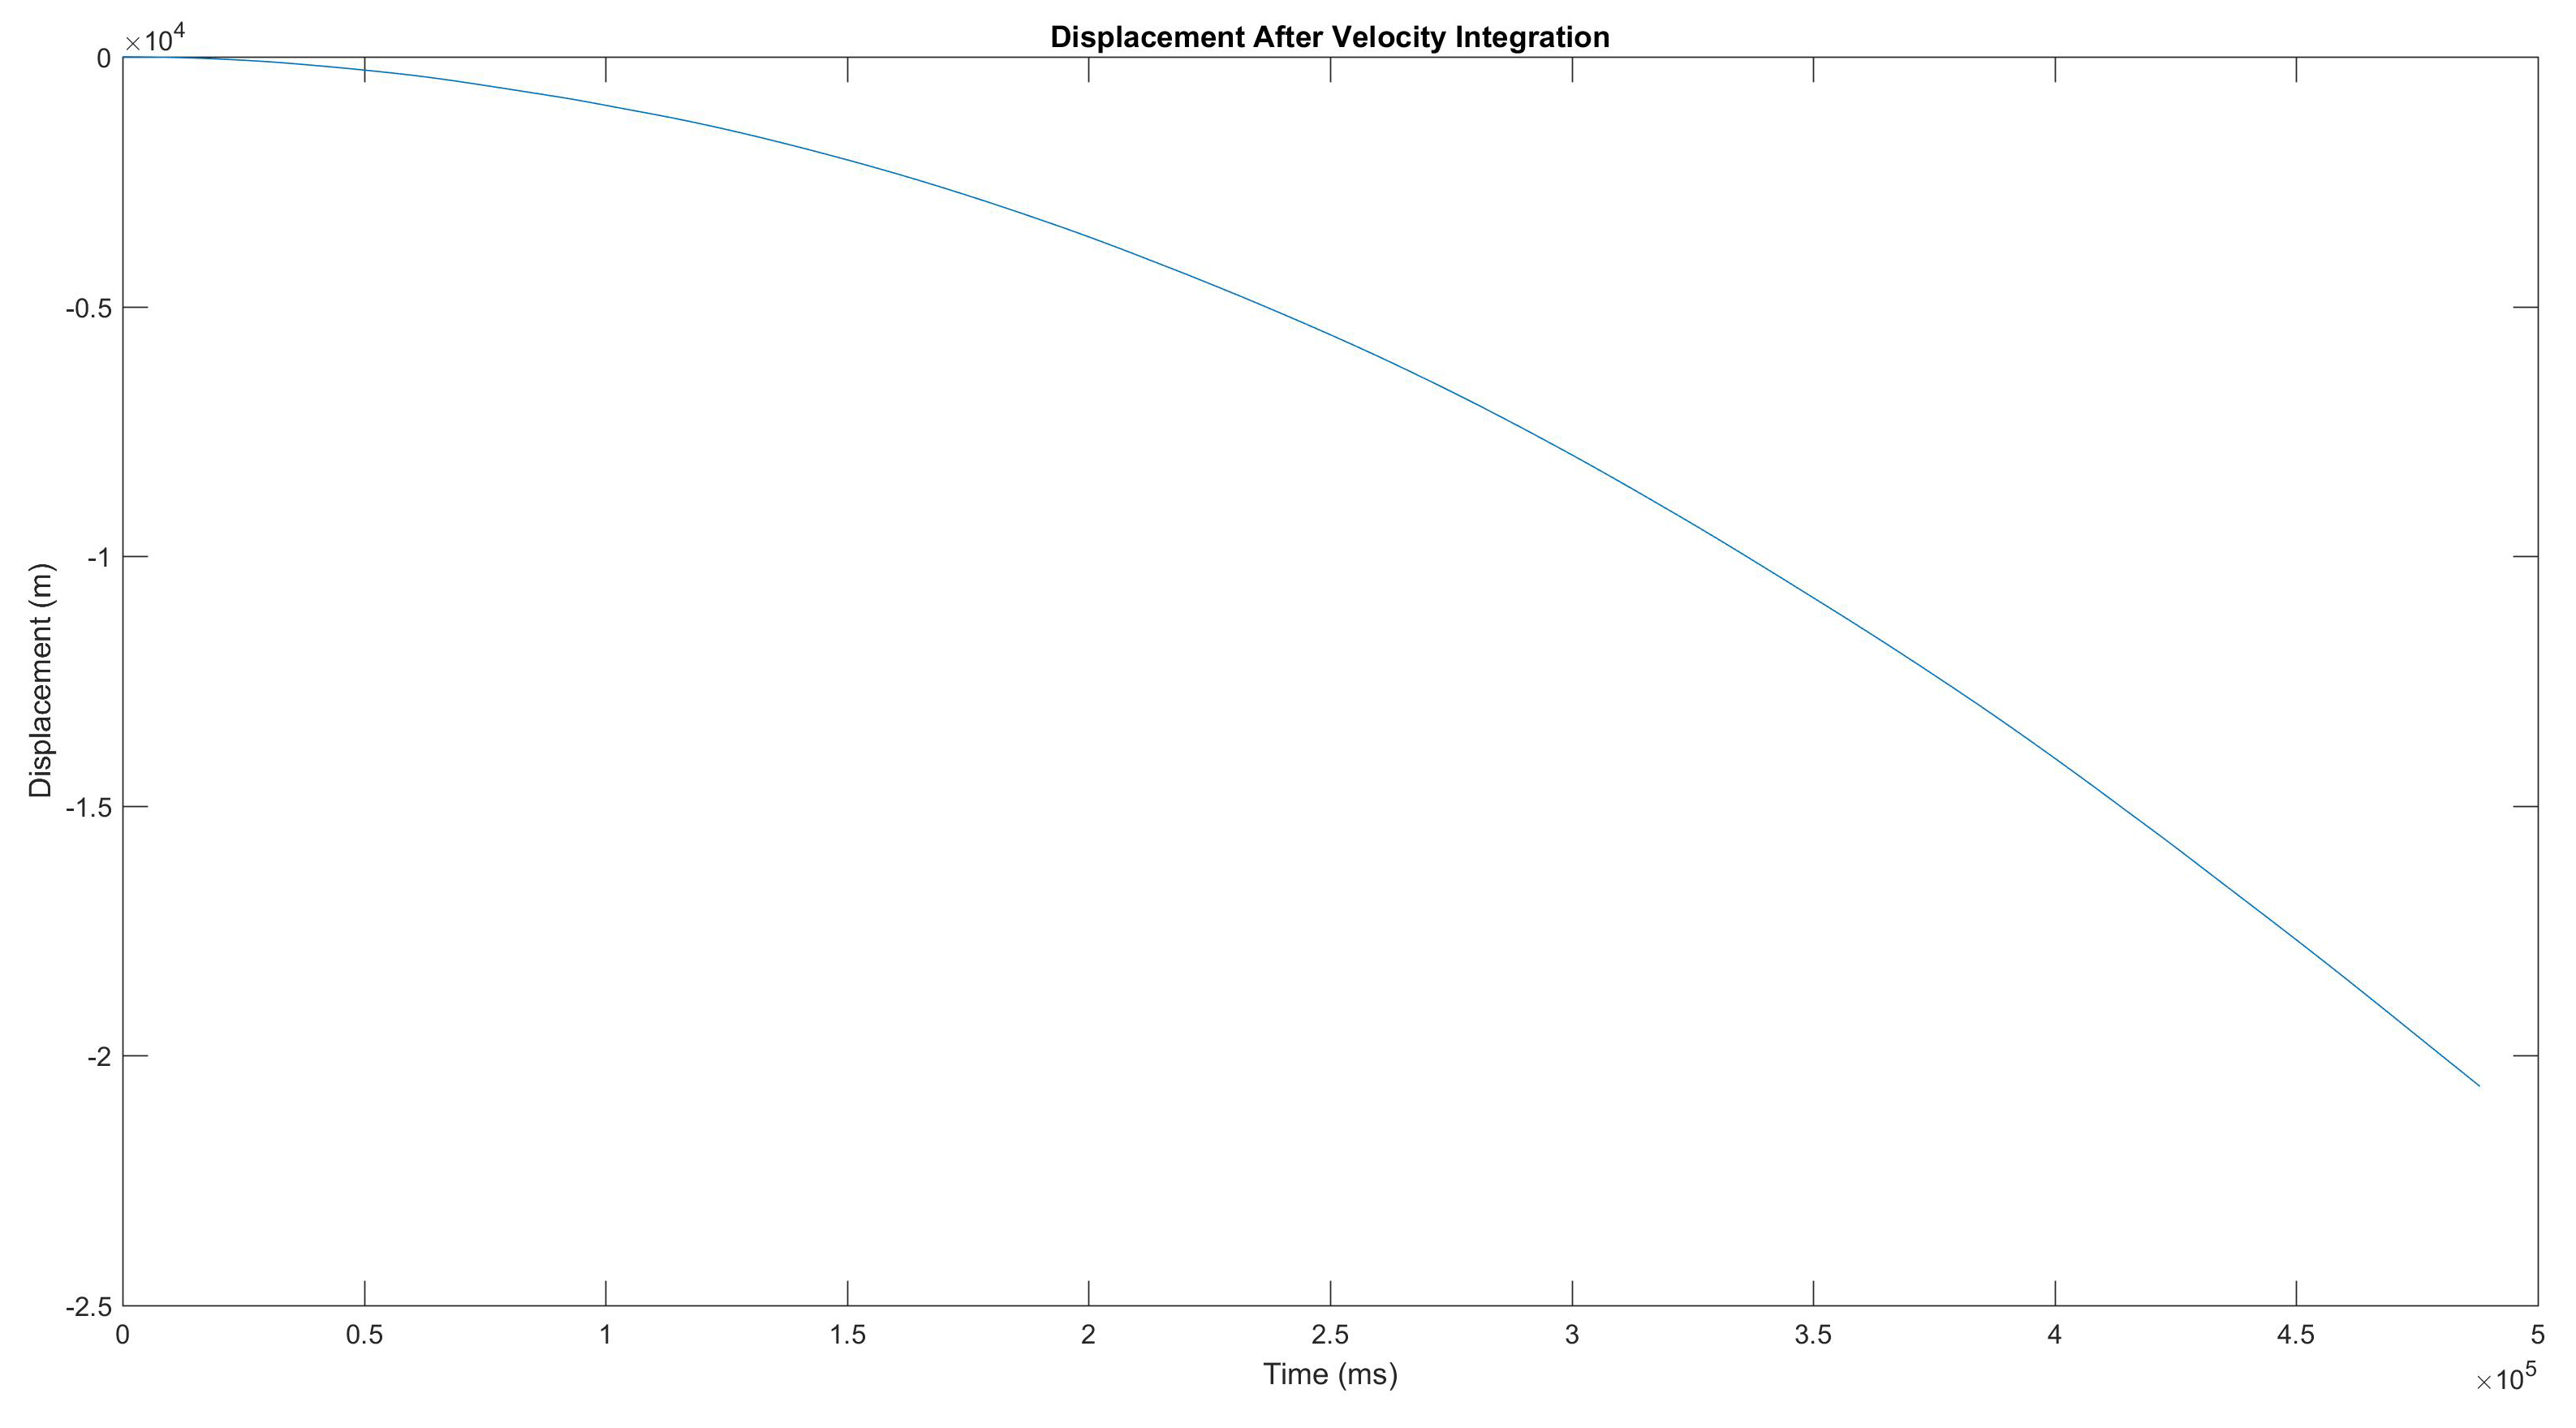
\includegraphics[scale=0.11]{DisplacementIntegration}\label{fig:Displacement}}  
  \caption{The result of double integration of a Raw Signal}
  \label{fig:Integration of Raw Data}
\end{figure}
\clearpage

\noindent As is possible see, the result is not realistic, considering it is vertical acceleration, so it is necessary to perform various steps to fix and clean the signal. First of all, the signal reorientation will be carried out respect the axes of the vehicle, and subsequently, various filter operations to clean the signal.

\section{Accelerometer Reorientation} \label{Accelerometer Reorientation}
\noindent The Cartesian reference system of the phone must be aligned with the vehicle reference system, to detect the vehicle motion correctly.
As shown in the figure below.

\begin{figure}[ht]
  \centering
  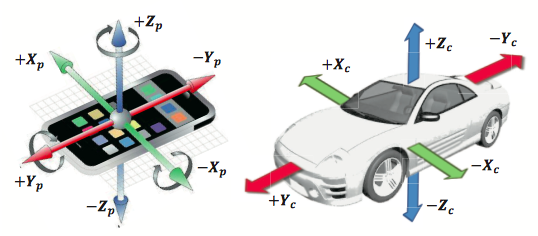
\includegraphics[scale=0.7]{phonecarorientation}  
  \caption{Correct alignment of smartphone respect to the vehicle cartesian frame.}
  \label{fig:Smartphone cartesian frame alignment respect Car axis.}
\end{figure}
\noindent Smartphone accelerometer detects the following accelerations: $a_{x_{p}}$ , $a_{y_{p}}$ and $a_{z_{p}}$ . To determine the accelerations felt by the vehicle and locate road surface anomalies. The accelerometer must detect what happens in the direction perpendicular ($Z$ axes) to the vehicle \cite{mohan2008nericell}.
Respectively the $X_{p}$ axis identifies the longitudinal direction, $Y_{p}$ axis the transverse direction and $Z_{p}$ the perpendicular direction respect to the $xy$ plane.

\noindent To detect road anomalies, the direction of the z-axis must correspond to the direction of the z axis. If this condition subsists, the accelerometer is well oriented, contrarily it is not well oriented and needs to be reoriented. But even if starting from a precise orientation condition, during travel the phone may be moving, or due to unexpected vehicle movements, travel of climbing, downhill, curve, all of these causes could affect the misalignment of the smartphone frame respect to the vehicle frame.

\noindent The reorientation can be performed by the Euler Angles. Three angles that allow to defining the orientation in space of any body through a succession of elementary rotations.\cite{diebel2006representing}
The $XYZ$ sequence was defined,a rotation around the $x$ axis by an angle $\alpha$ (roll angle), one around the $y$ axis by $\beta$ (pitch angle) and one around the $z$ axis by  $\gamma$ (yaw angle).\\\\
\noindent The equations that allows to reoriented data by the $\alpha$, $\beta$, $\gamma$, angle are:\cite{Andro}
\begin{equation}
a_{x_{reor}} = \cos (\beta) a_{x_{p}} + \sin (\beta) \sin (\alpha) a_{y_{p}} + \cos (\alpha) \sin (\beta) a_{z_{p}} 
\end{equation}
\begin{equation}
a_{y_{reor}} = \cos (\alpha) a_{y_{p}} - \sin (\alpha) a_{z_{p}}
\end{equation}
\begin{equation}
a_{z_{reor}} = -\sin (\beta) a_{x_{p}} + \cos (\beta) \sin (\alpha) a_{y_{p}} + \cos (\beta) \cos (\alpha) a_{z_{p}}
\end{equation}


\noindent The figure below, show an example of reoriented data.
\begin{figure}[ht]
  \centering
  \subfloat[Raw]{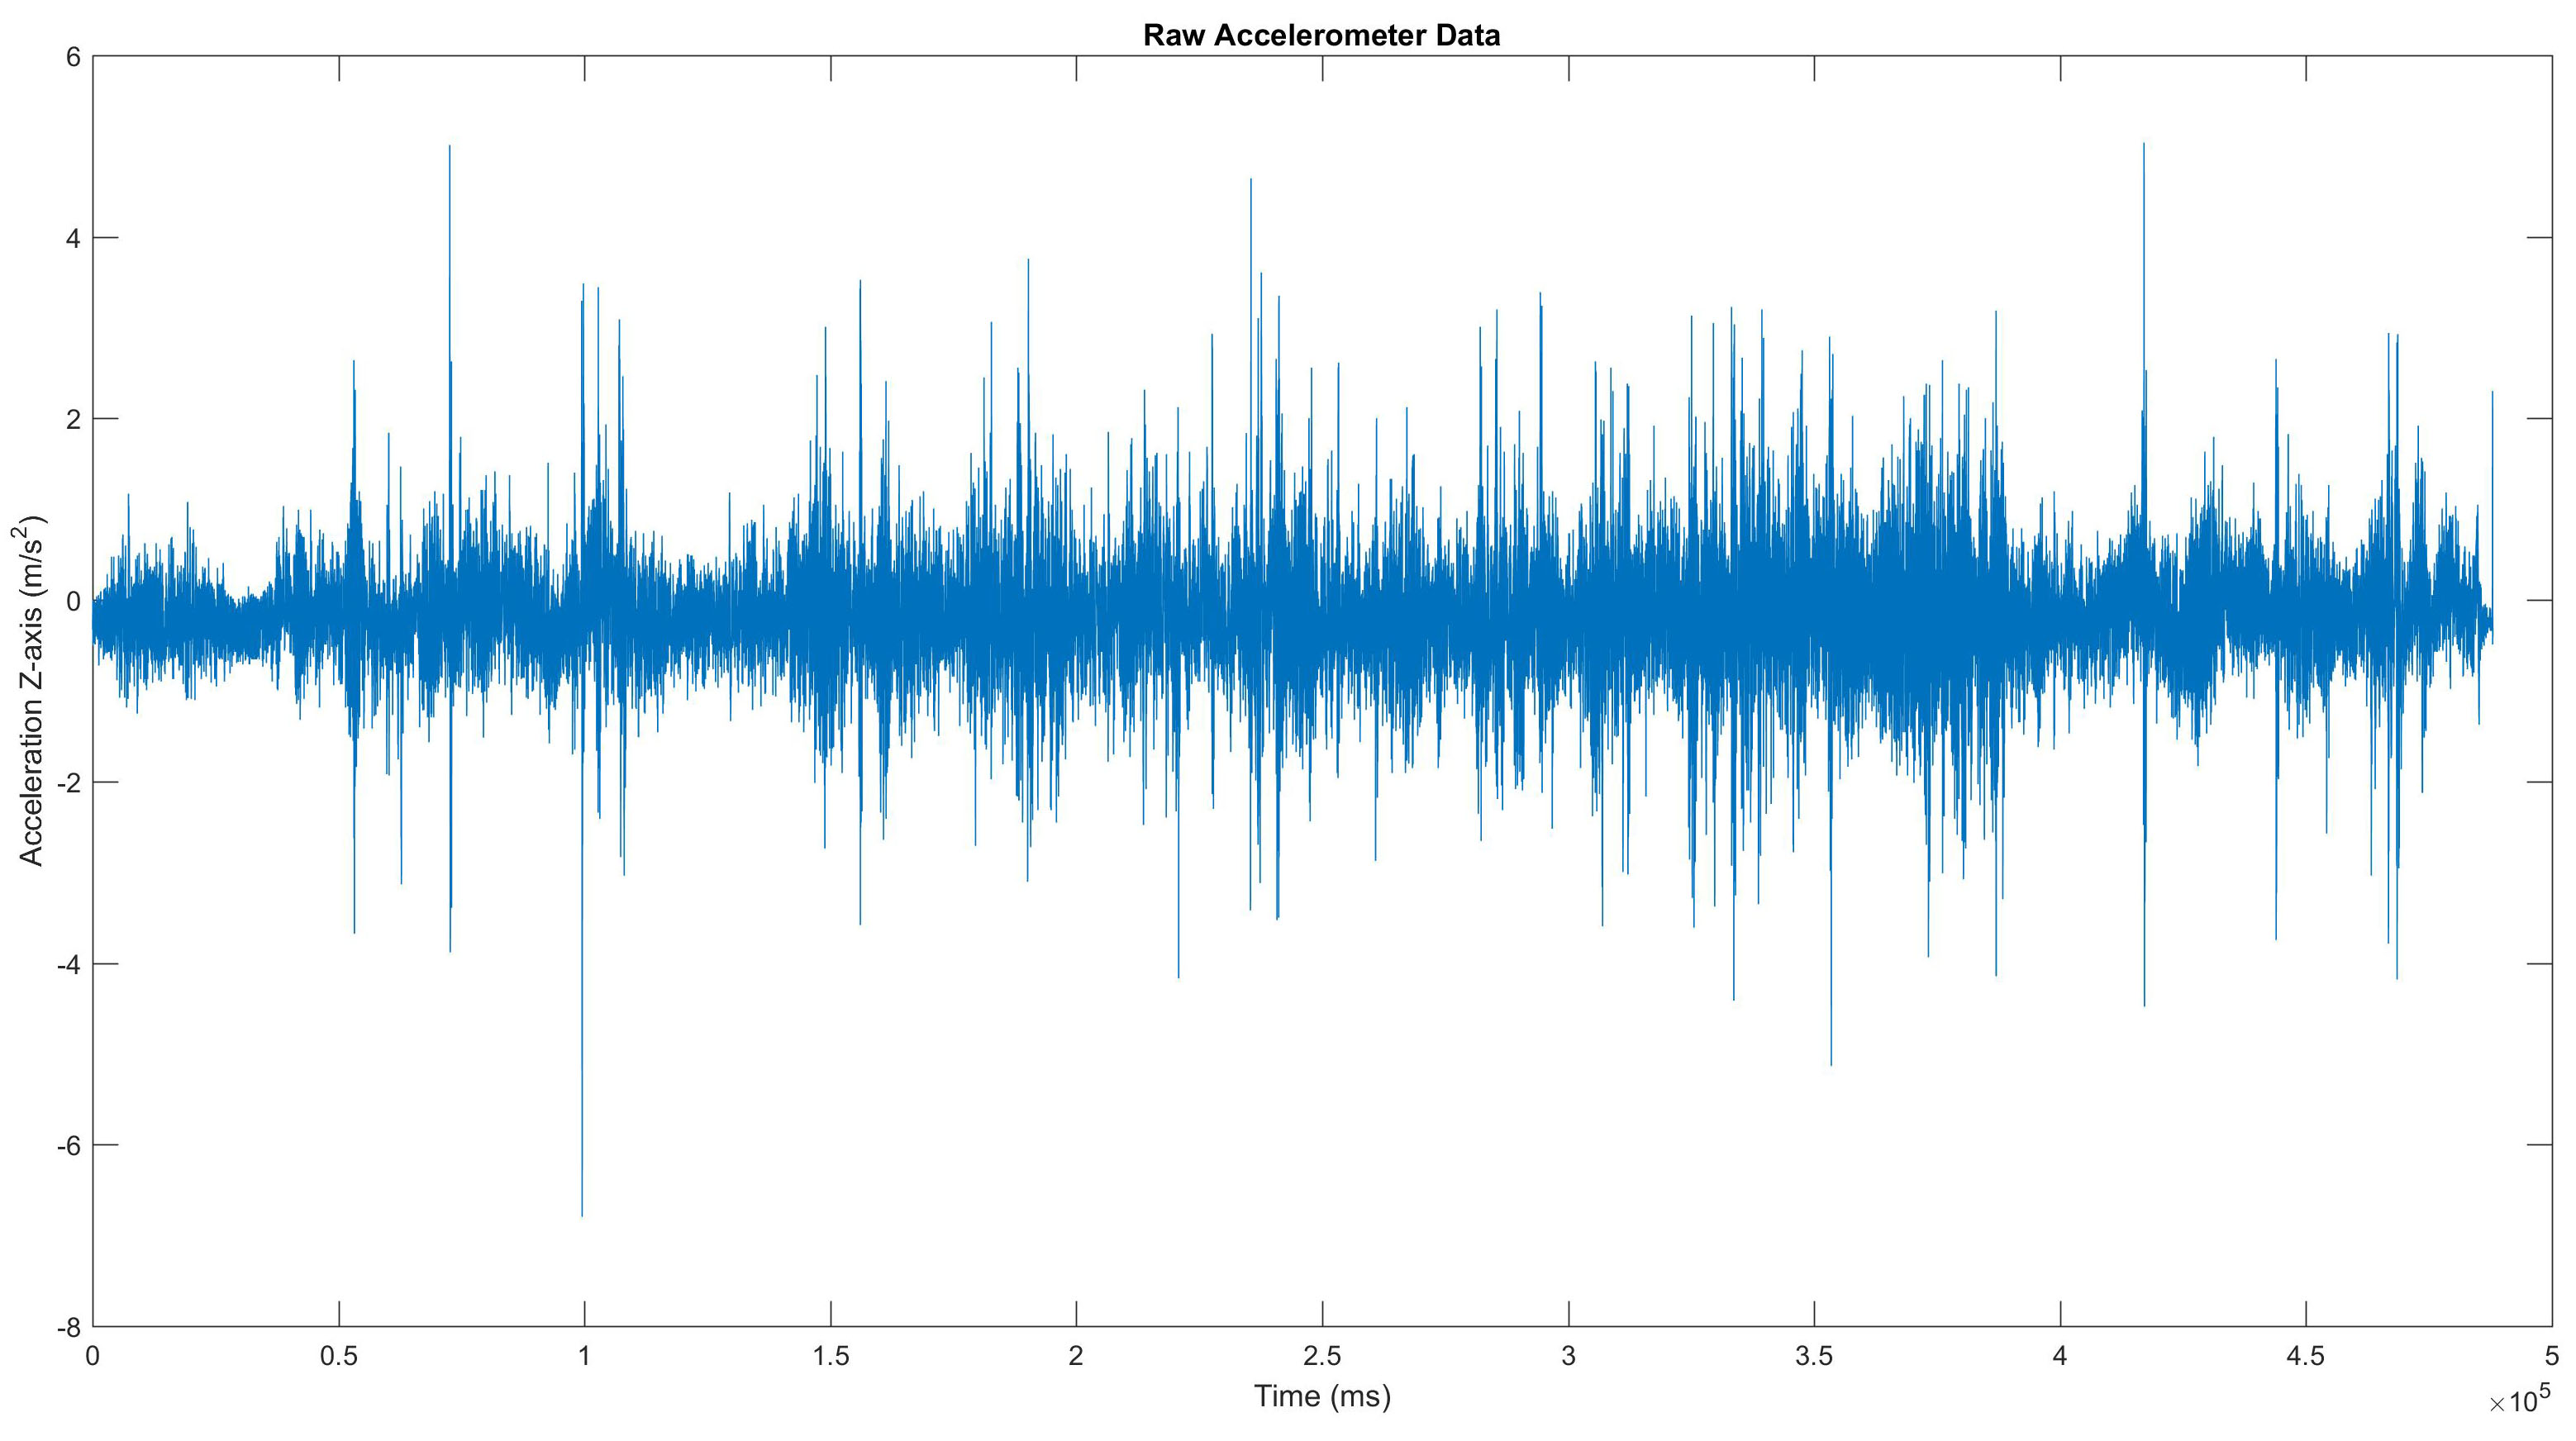
\includegraphics[scale=0.11]{raw}\label{fig:Raw Accelerometers}}  
  
  \subfloat[Reoriented]{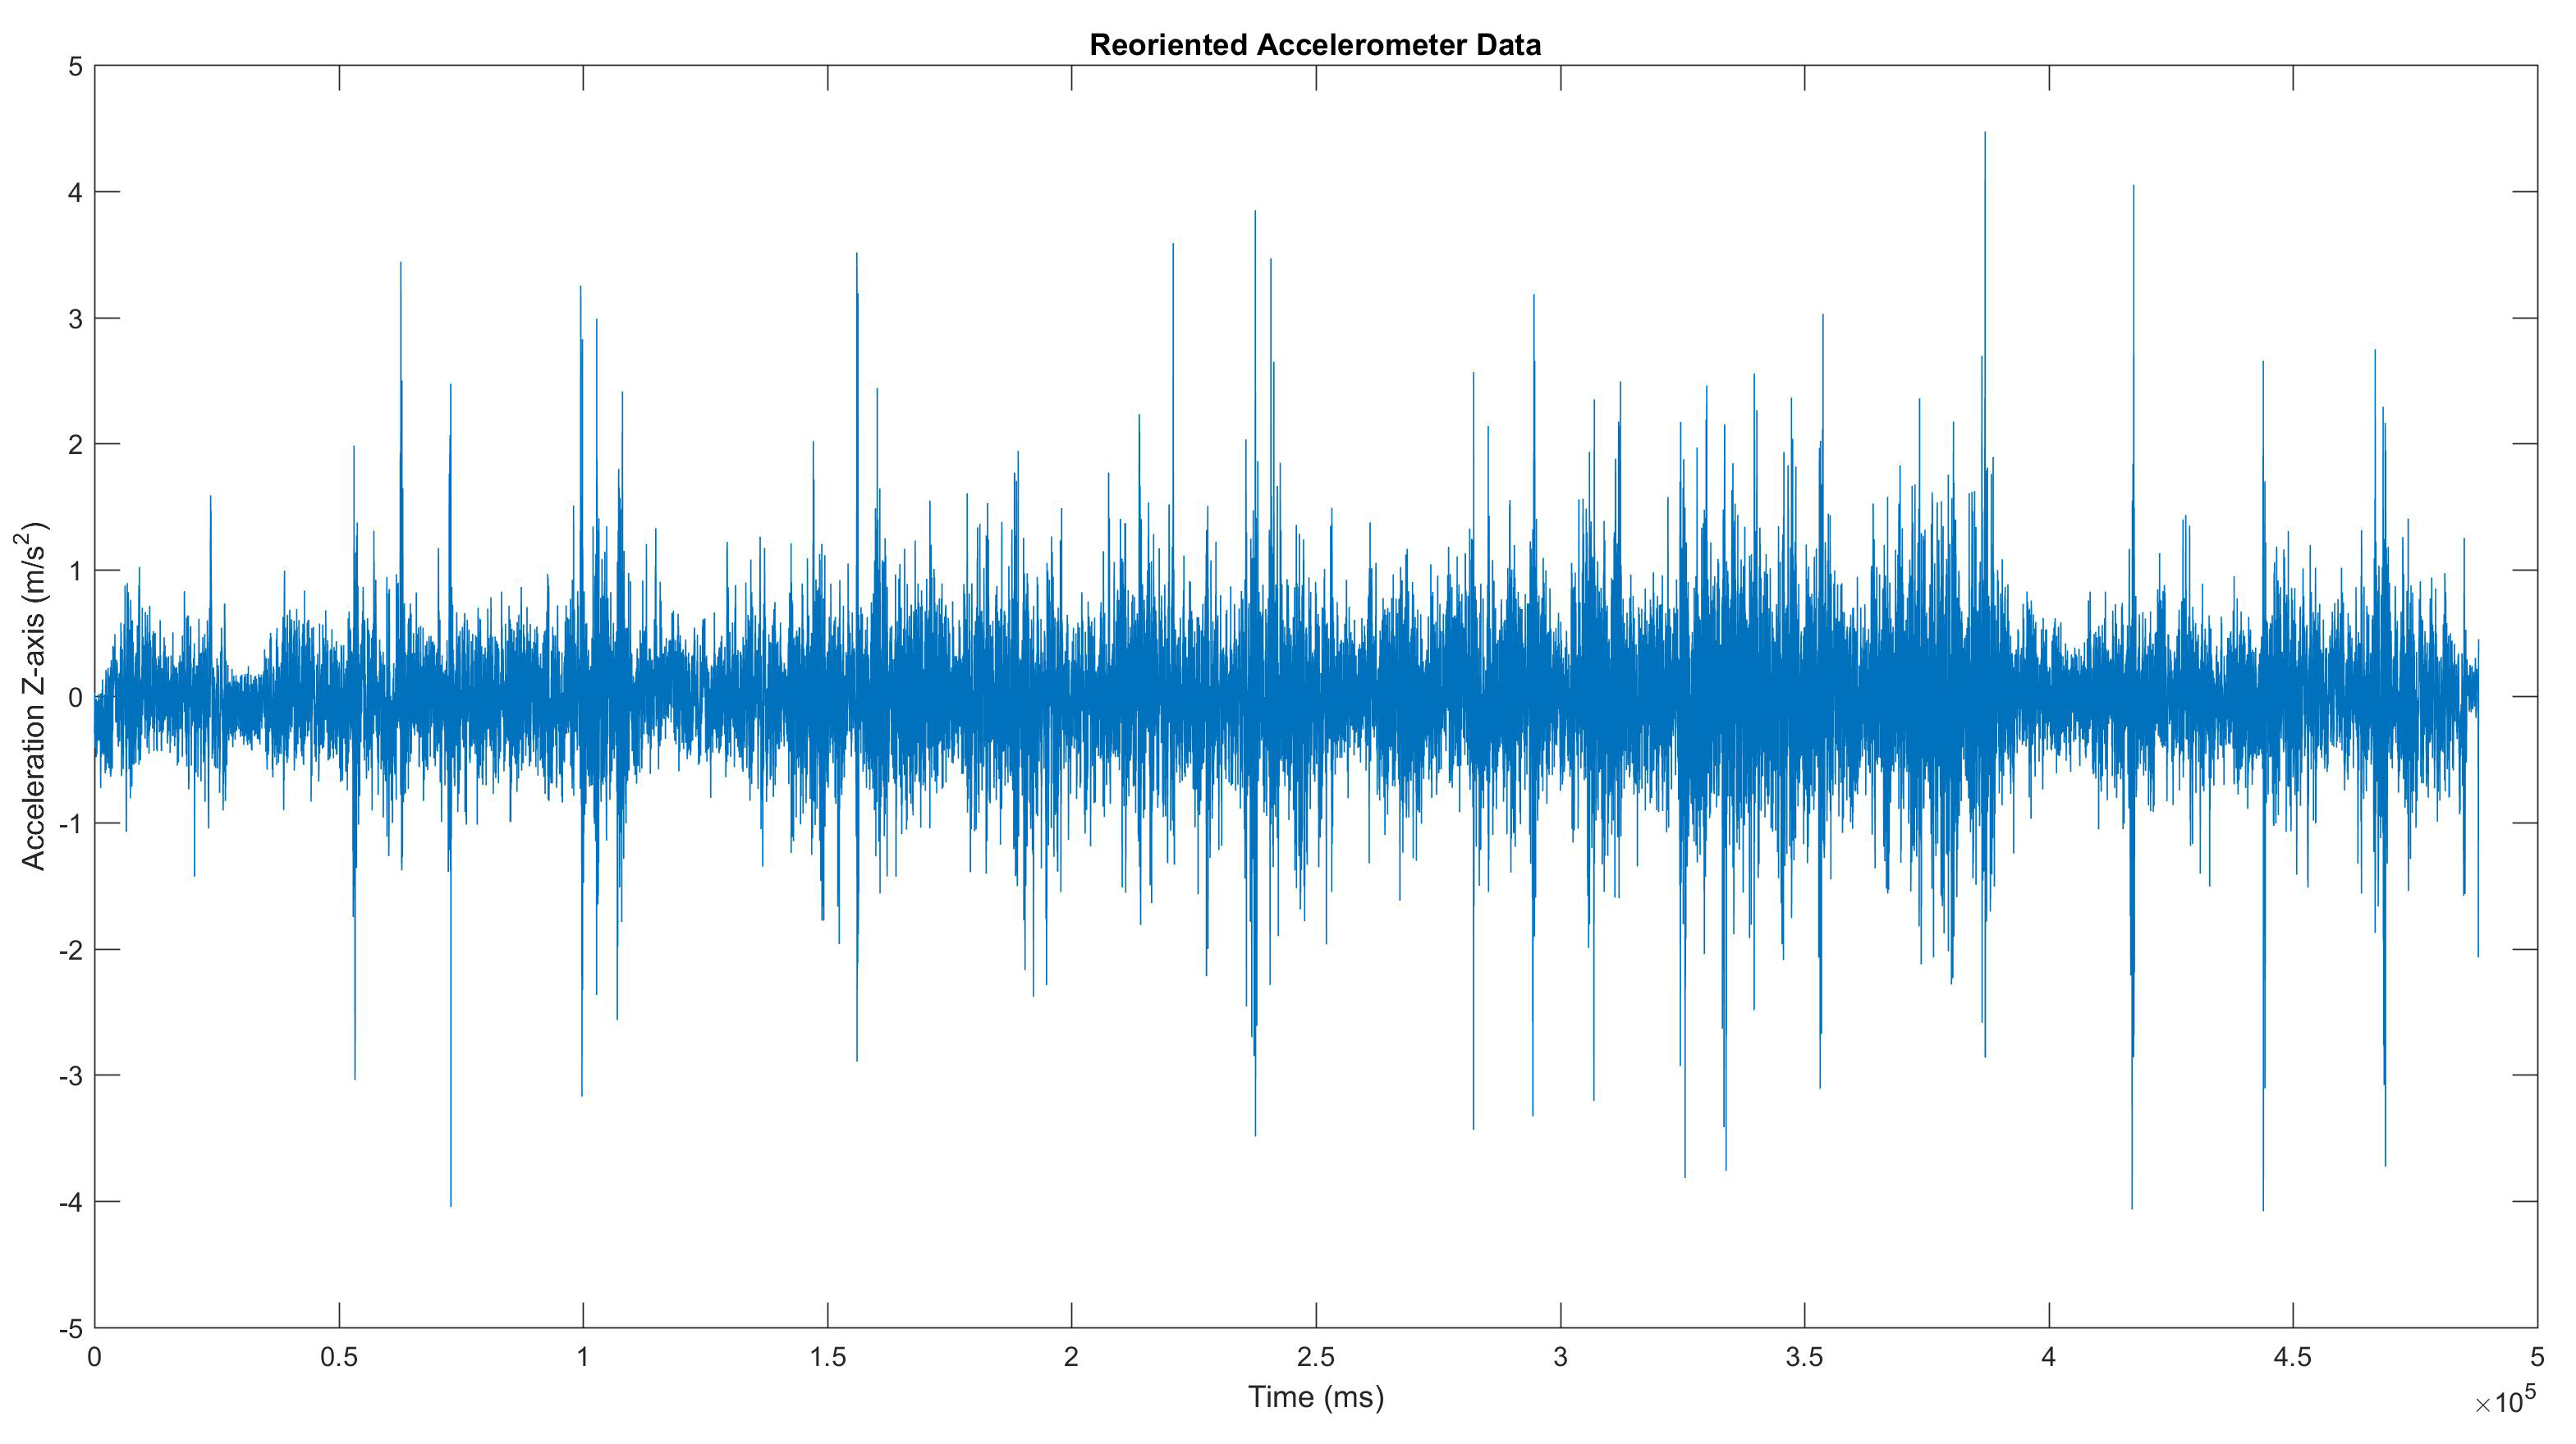
\includegraphics[scale=0.11]{reoriented}\label{fig:Reoriented Accelerometer}}

 
  \caption{The result of reorientation of raw data}
  \label{fig:Accelerometer Reoriented}
\end{figure}

\end{document}